
\begin{enumerate}
%%%%%%%%%
\item  Gracias a los esteres y algunos compuestos aromáticos es posible percibir el olor de las frutas y de las flores, por esto son utilizados para la elaboración de esencias, aromatizantes, perfumes. La esencia de naranja es el acetato de octilo el cual corresponde a la siguiente fórmula: \label{jenn-1}


\begin{enumerate}[(A)]
\item CH$_3$-CH$_2$-COO-(CH$_2$)$_6$-CH$_3$
\item CH$_3$-COO-(CH$_2$)$_7$-CH$_3$
\item CH$_3$-CH$_2$-COO-(CH$_2$)$_5$-CH$_3$
\item CH$_3$-(CH$_2$)$_6$-COO-CH$_2$-CH$_3$
\end{enumerate}
%%%%%%%%%%%%%%%%%%%%%%%%%%%%%


\item  La fuerza que mantiene unidos los átomos entre sí, se le llama enlace químico, el cual le confiere ciertas propiedades a los compuestos formados. De acuerdo con lo anterior son propiedades de los compuestos iónicos:\label{jenn-3}


\begin{enumerate}[(A)]
\item   sólidos a temperatura ambiente y altos puntos de fusión.
\item buenos conductores de la electricidad y poseen brillo metálico.
\item bajos puntos de fusión y de ebullición.
\item malos conductores del calor y la electricidad.
\end{enumerate}

%%%%%%%%%%%%%%%%%%%%%%%%%%%%%

\newpage
\item La lactosa, azúcar de la leche, es un disacárido, constituido por una molécula de glucosa y una de galactosa. Algunas personas pueden ser intolerantes a este carbohidrato debido a la ausencia de la enzima lactasa, y por ello deben consumir productos deslactosados. Una de las siguientes estructuras corresponde a la lactosa. \label{jenn-2}
\begin{enumerate}[(A)]
\item 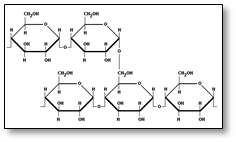
\includegraphics[width=0.3\textwidth]{img1.png}
\item 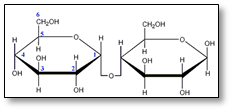
\includegraphics[width=0.3\textwidth]{img2.png}
\item 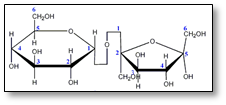
\includegraphics[width=0.3\textwidth]{img3.png}\\
\item 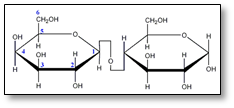
\includegraphics[width=0.3\textwidth]{img4.png}
\end{enumerate}





%%%%%%%%%%%%%%%%%%%%%%%%%%%%%

\newpage
\item  Según el modelo atómico de Bohr, la representación correcta para un elemento que se encuentra ubicado en el grupo IIIA, periodo 3 es:\label{jenn-4}


\begin{enumerate}[(A)]
\item 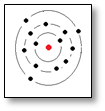
\includegraphics[width=0.25\textwidth]{img5.png}
\item 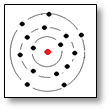
\includegraphics[width=0.25\textwidth]{img6.png}
\item 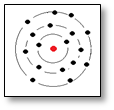
\includegraphics[width=0.25\textwidth]{img7.png}\\
\item 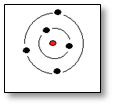
\includegraphics[width=0.25\textwidth]{img8.png}
\end{enumerate}


%%%%%%%%%%%%%%%%%%%%%%%%%%%%%

\newpage
\item   La estructura de Lewis son representaciones de los enlaces químicos, la cual permite explicar la tendencia de los átomos a completar con ocho electrones su última capa. De acuerdo con la anterior información la estructura correcta para el compuesto BCl$_3$ es:\label{jenn-5}


\begin{enumerate}[(A)]
\item 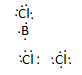
\includegraphics[width=0.22\textwidth]{img9.png}
\item 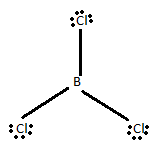
\includegraphics[width=0.25\textwidth]{img10.png}
\item 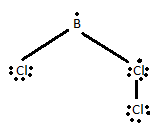
\includegraphics[width=0.25\textwidth]{img11.png}\\
\item 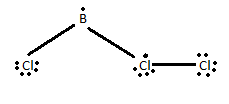
\includegraphics[width=0.30\textwidth]{img12.png}
\end{enumerate}


%%%%%%%%%%%%%%%%%%%%%%%%%%%%%


\item En la etiqueta de un vino tinto se especifica que este contiene un 13.5 \% de volumen en alcohol, esto quiere decir que el vino contiene:\label{jenn-6}


\begin{enumerate}[(A)]
\item 13.5 g de alcohol por cada 100 mL 
\item  13.5 g de alcohol por cada 100 g
\item  13.5 mL de alcohol por cada 100 mL
\item  13.5 mL de alcohol por cada 100O mL
\end{enumerate}


%%%%%%%%%%%%%%%%%%%%%%%%%%%%%

\subsubsection*{Conteste las preguntas \ref{jenn-7} y \ref{jenn-8} de acuerdo con la siguiente información.}

 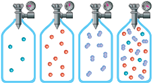
\includegraphics[width=0.45\textwidth]{img13.png}

Respectivamente T = 20$^o$C, H2 = 1 atm, Ar = 3 atm, CO2 = 1 atm.



\item  La temperatura y el volumen que se obtiene al mezclarse los gases en el nuevo cilindro es de:\label{jenn-7}


\begin{enumerate}[(A)]
\item 20$^o$C y 3L
\item  60$^o$C y 3L
\item  60$^o$C y 1L
\item  20$^o$C y 1L
\end{enumerate}


%%%%%%%%%%%%%%%%%%%%%%%%%%%%%


\item Según la teoría de Dalton la presión total de los tres gases al mezclarse es de: \label{jenn-8}


\begin{enumerate}[(A)]
\item    5 atm
\item  1 atm
\item  3 atm
\item  2 atm
\end{enumerate}


%%%%%%%%%%%%%%%%%%%%%%%%%%%%%


\item  El propanoato de calcio es una sal cálcica de fórmula Ca(C2H5COO)2, utilizada como conservante en la elaboración de algunos productos alimenticios como el pan blanco. El grupo funcional al que pertenece es:\label{jenn-9}


\begin{enumerate}[(A)]
\item Acido carboxílico
\item Aldehído
\item Cetona
\item Éster 
\end{enumerate}


%%%%%%%%%%%%%%%%%%%%%%%%%%%%%


\item  La cerveza es una bebida de sabor amargo, producto de la fermentación anaerobia de cereales como la cebada, que por medio de microorganismos como la levadura procesan los carbohidratos como (glucosa, fructosa, sacarosa, almidón entre otros) para obtener alcohol y dióxido de carbono. La reacción que se lleva a cabo en la fermentación alcohólica es la siguiente: C$_6$H$_12$O$_6$ + 2 ADP $\longrightarrow$ 2 CH$_3$-CH$_2$OH + 2 CO$_2$ + 2 ATP + 25.5 kcal \label{jenn-10}\\
De acuerdo con la siguiente información el alcohol que se obtiene es:


\begin{enumerate}[(A)]
\item Etanol
\item Metanol
\item Alcohol propílico
\item Alcohol metílico
\end{enumerate}


%%%%%%%%%%%%%%%%%%%%%%%%%%%%%


\item Según la gráfica de la curva de valoración entre el HCl (un ácido fuerte) y el NaOH (una base fuerte), 
 \label{jenn-11}


\item 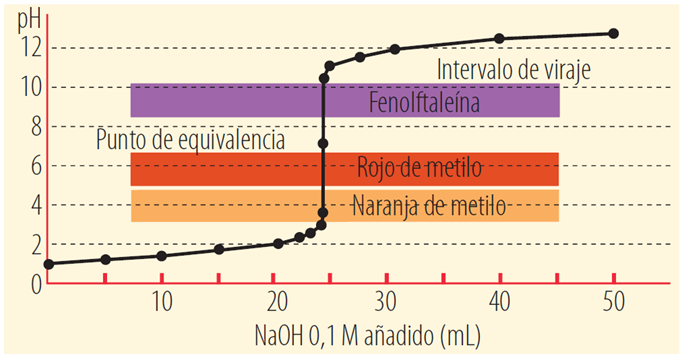
\includegraphics[width=0.45\textwidth]{img14.png}

El indicador que deja observar claramente el punto de equivalencia en la titulación es:

\begin{enumerate}[(A)]
\item   fenolftaleína
\item rojo de metilo
\item naranja de metilo
\item ninguna de las anteriores
\end{enumerate}


%%%%%%%%%%%%%%%%%%%%%%%%%%%%%


\newpage
\item  Para la titulación de 25 mL de ácido acético (CH$_3$COOH) se necesitaron 36 mL de hidróxido de potasio (KOH) 0.2 N ¿Cuál es la concentración del ácido acético? \label{jenn-12}


\begin{enumerate}[(A)]
\item   0.3N 
\item 0.5N
\item 1N
\item 0.2N
\end{enumerate}


%%%%%%%%%%%%%%%%%%%%%%%%%%%%%

\item  Para la siguiente reacción  \label{jenn-13}

\begin{equation*}
C_{11}H_{22}O_{11}+O_{2}\longrightarrow CO_{2}+H_{2}O
\end{equation*}

El balanceo correspondiente es,
\begin{enumerate}[(A)]
\item   1;33;11;11
\item 1;11;11;11
\item 1;2;11;22
\item 1;2 ;11;2
\end{enumerate}


%%%%%%%%%%%%%%%%%%%%%%%%%%%%%


\item   La IUPAC es el la Unión Internacional de Química Pura y Aplicada, encargada de establecer las reglas para nombrar los compuestos químicos orgánicos e inorgánicos. De acuerdo a lo anterior el NaClO4, se conoce como:\label{jenn-14}


\begin{enumerate}[(A)]
\item   perclorato de sodio
\item clorato de sodio
\item hipoclorito de sodio
\item clorito de sodio
\end{enumerate}


%%%%%%%%%%%%%%%%%%%%%%%%%%%%%


\item Una reacción de desplazamiento o sustitución es aquella en la que un elemento sustituye y libera a otro elemento presente en el compuesto. De acuerdo con esta información es una reacción de desplazamiento,  \label{jenn-15}


\begin{enumerate}[(A)]
\item $2KClO_{3}\longrightarrow 2KCl + 3O_{2}$
\item $As_{2}O_{3}+4HNO_{3}+H_{2}O$\\ 
 $\longrightarrow\ 2H_{3}AsO_{4}+4NO_{2}$\hfill
\item $Zn + CuSO_{4}+H_{2}O\longrightarrow Cu + ZnSO_{4}$
\item $NaCl+AgNO_{3}\longrightarrow AgCl + NaNO_{3}$
\end{enumerate}


%%%%%%%%%%%%%%%%%%%%%%%%%%%%%


\item  Para las siguientes reacciones, \label{jenn-16}

\begin{align*}
R+O_{2}&\longrightarrow N\\
N+H_{2}O&\longrightarrow U\\
U+HX&\longrightarrow Z+H_{2}O
\end{align*}

De acuerdo con lo anterior $X$ es un no metal, $Z$ es una sal y $U$ es, oxido acido

\begin{enumerate}[(A)]
\item   Oxido básico
\item Ácido oxácido
\item Hidróxido
\end{enumerate}


%%%%%%%%%%%%%%%%%%%%%%%%%%%%%


\item En el compuesto Cl$_2$O$_3$, los estados de oxidación del cloro y del oxígeno son respectivamente, \label{jenn-17}


\begin{enumerate}[(A)]
\item   -2, +2   
\item +2, -2                         
\item -3, +2    
\item   +3, -2
\end{enumerate}


%%%%%%%%%%%%%%%%%%%%%%%%%%%%%


\item  La tabla muestra el porcentaje en peso de unos iones presentes en dos muestras de agua tomados de dos lugares diferentes,\label{jenn-18}

\begin{center}
\begin{tabular}{c|cc}
\hline 
\hline 
 & \multicolumn{2}{c}{Porcentaje en peso}   \\ 
Iones & Muestra 1 & Muestra 2 \\ 
\hline 
\hline 
K$^{+}$ & 4.25 & 0 \\		 
Na$^{++}$ & 6.36 & 0 \\ 
Ca$^{++}$ & 7.38 & 0 \\ 
Cl$^{-}$ & 16.25 & 12.00 \\ 
\hline 
\end{tabular} 
\end{center}

\begin{enumerate}[(A)]
\item   CaNa$_2$; CaK$_2$; CaCl$_2$
\item NaK; CaCl$_2$; NaKCl
\item NaCl; KCl; CaCl$_2$
\item NaCa; KCa; KCl$_2$
\end{enumerate}


%%%%%%%%%%%%%%%%%%%%%%%%%%%%%

\newpage
\item  La isomería es una propiedad de los compuestos químicos, en el cual se presenta una misma fórmula molecular pero con estructura u organización diferente de los átomos. De este modo es un isómero del ácido 2-hidroxihexanoico \label{jenn-19}


\begin{enumerate}[(A)]
\item 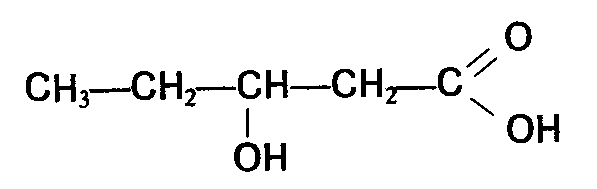
\includegraphics[width=0.35\textwidth]{img15.png}
\item 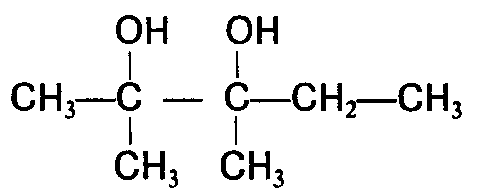
\includegraphics[width=0.32\textwidth]{img16.png}
\item 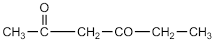
\includegraphics[width=0.38\textwidth]{img17.png}\\
\item 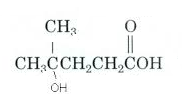
\includegraphics[width=0.3\textwidth]{img18.png}
\end{enumerate}


%%%%%%%%%%%%%%%%%%%%%%%%%%%%%


\item La aspirina o acido acetilsalicilico, es uno de los principales analgesicos a nivel mundial, \label{jenn-20}

\begin{center}
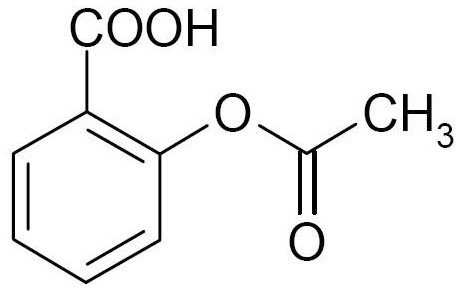
\includegraphics[width=0.30\textwidth]{img19.jpeg}
\end{center}

Químicamente, las funciones que integran la estructura de la aspirina es,


\begin{enumerate}[(A)]
\item   Benceno, éster y acido carboxílico
\item Fenol, cetona y acido carboxílico
\item Aldehído, éter y benceno
\item Aldehído, cetona y benceno
\end{enumerate}


%%%%%%%%%%%%%%%%%%%%%%%%%%%%%


\item El reactivo de Lugol es una disolución entre yodo molecular (I2) y yoduro potásico (KI), el cual es utilizado para la identificación de polisacáridos como el almidón. ¿Por qué el reactivo de Lugol presenta una coloración azul oscura o negra en presencia de almidón? \label{jenn-21}\hrulefill\\
\_\hrulefill\\
\_\hrulefill\\
\_\hrulefill.



%%%%%%%%%%%%%%%%%%%%%%%%%%%%%


\item   ¿Qué diferencia hay entre una solución homogénea y un coloide?\label{jenn-22}\hrulefill\\
\_\hrulefill\\
\_\hrulefill\\
\_\hrulefill.


%%%%%%%%%%%%%%%%%%%%%%%%%%%%%


\item ¿Qué es un polímero? \label{jenn-23}\hrulefill\\
\_\hrulefill\\
\_\hrulefill\\
\_\hrulefill.



%%%%%%%%%%%%%%%%%%%%%%%%%%%%%


\item  Los aldehídos presentan reacciones de oxidación, de acuerdo con la anterior información si se oxida el 2-metil-hexanal¿ Cuál es el compuesto que se forma \label{jenn-24}\hrulefill\\
\_\hrulefill\\
\_\hrulefill\\
\_\hrulefill.





%%%%%%%%%%%%%%%%%%%%%%%%%%%%%


\item  En la determinación de la cantidad de sustancia que se produce durante una reacción química, es necesario conocer el reactivo limite, ¿Por qué es necesario conocerlo?
\label{jenn-25}\hrulefill\\
\_\hrulefill\\
\_\hrulefill\\
\_\hrulefill.








%%%%%%%%%%%%%%%%%%%%%%%%%%%%%
\end{enumerate}
%%%%%%%%%%%%%%%%%%%%%%%%%%%%%5
